\documentclass{article}
\usepackage[]{amsmath}
\usepackage[]{amsfonts}
\usepackage[]{framed}
\usepackage[]{parallel}
\usepackage[]{siunitx}
\usepackage[colorlinks=true,
urlcolor=blue]{hyperref}
\usepackage[]{tikz}
\usepackage[]{fullpage}
\usetikzlibrary{positioning}
\DeclareFontFamily{U}{wncy}{}
\DeclareFontShape{U}{wncy}{m}{n}{<->wncyr10}{}
\DeclareSymbolFont{mcy}{U}{wncy}{m}{n}
\DeclareMathSymbol{\Sh}{\mathord}{mcy}{"58}
\begin{document}
\input{measurement.tex}
\section{Periodicity Considerations}
\label{sec:periodicity_considerations}

\begin{framed}
   Performing a IDFT on the measured VNA data should use a periodic time-domain
   input because the DFT is a periodic transform.
\end{framed}

As acknowledged in Phillip Dunsmore's thesis
(\url{http://etheses.whiterose.ac.uk/3355/1/uk_bl_ethos_406207.pdf}) a periodic
transform imposes periodic functions on the analysis. The discrete Fourier
transform is such a periodic transform. Thus, both the time-domain response and
the frequency-domain response must be considered periodic. Quoting the thesis:
``The step response of the VNA should retain the property that its derivative is
the VNA time-domain impulse response, and since the sampling function [the VNA
being the sampler] creates a periodic time-domain, with a period of $
\frac{1}{\Delta \omega} $, the step response should retain this aspect of the
periodicity.'' From here, the author determines the requirements of the step
response given the required periodicity of the impulse response. And herein lies
an important detail: The step response is the sum of two responses, one is a
periodic portion (responsible for the periodicity of the impulse response); the
other part is a ramp portion (staircase), which is responsible for the impulses
within the impulse response. However, since this is not in $ L^2 $, a Laplace
transform is used for the ramp portion and a Fourier transform is used for the
periodic portion.

I think the above detail may be incredibly relevant.

\section{Methods of Implementation}
\label{sec:methods of implementation}

This section will outline the various approaches that I'm using to solve this
problem. Where appropriate, I will indicate which Git branch I am using for each
implementation.
\subsection{Na\"{i}ve Implementation - [master]}
\label{sub:naive_implemenation_master}



In this approach, the idea is simple:

\begin{enumerate}
  \item DFT the time-domain signal whose response you're
    interested in, obtaining the analytic frequency-domain function
    \subitem $\mathcal{FFT}(v(t)) = S(\omega)$.
  \item Multiple the VNA data and the sampled version of the signal (frequency
    domain) to obtain the response
    \subitem $ S(\omega)\textrm{VNA}(\omega) = R(\omega) $
  \item Invert the response to obtain the time-domain version:
    \subitem $\mathcal{DFT}^{-1}(R(w)) = r(t)$
\end{enumerate}

Variations on this involve using $S(w) = 1$ (a delta function in time) and
convolving the "impulse response" with the time-domain signal $ s(t) $.

\begin{figure}[h]
  \centering
  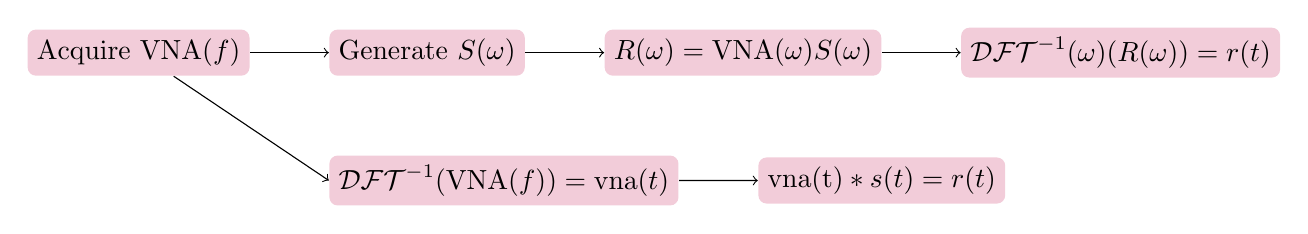
\begin{tikzpicture}
    [scale=.8,auto=left,every node/.style={rectangle,fill=purple!20,rounded
    corners=3pt}]
    % upper branch
    \node (a) at (0,0) {Acquire $ \textrm{VNA}(f) $};
    \node (b) [right=of a] {Generate $S(\omega)$};
    \node (c) [right=of b] {$R(\omega) = \textrm{VNA}(\omega)S(\omega)$};
    \node (d) [right=of c] {$\mathcal{DFT}^{-1}(\omega)(R(\omega)) = r(t)$};
    \draw[->] (a) -- (b); \draw[->] (b) -- (c); \draw[->] (c) -- (d);
    % Lower branch
    \node (e) [below right=of a] {$ \mathcal{DFT}^{-1}(\textrm{VNA}(f)) =
      \textrm{vna}(t) $};
    \node (f) [right=of e] {$ \textrm{vna(t)} * s(t) = r(t)$};
    \draw[->] (a) -- (e.west); \draw[->] (e) -- (f);
  \end{tikzpicture}
  \caption{Workflow for approach 1.}
  \label{fig:approach_1_graph}
\end{figure}

\subsubsection{Caveats: Approach 1}
\label{sub:caveats_approach_1}

\begin{enumerate}
  \item VNA data is assumed to be periodic, but $ S(\omega) $ is not periodic
    ($\mathcal{F}$).
  \item Time-domain points (spacing, number) are constrained by the frequency-domain points.
\end{enumerate}

\subsection{Phillip Dunsmore's Approach - [pdunsmore]}
\label{sub:phillip_dunsmore_s_approach_pdunsmore_}

Phillip Dunsmore's thesis provides a mathematical framework for approaching this
problem. His solution most differs from the na\"{i}ve solution in that the VNA
data is assumed to have been acquired as if a sampling function was applied to
the frequency domain. He uses the sampling function $\Sh(f)$ to pluck off
frequency components. He accounts for the finite frequency domain by applying a
rectangular filter function $\Theta(f_{max})$ to the measured data.

Concretely,

\begin{enumerate}
  \item
\end{enumerate}

\end{document}
